\documentclass{article}
\usepackage[utf8]{inputenc}
\usepackage{tikz}
\usetikzlibrary{positioning}
\usetikzlibrary{shapes}

\begin{document}

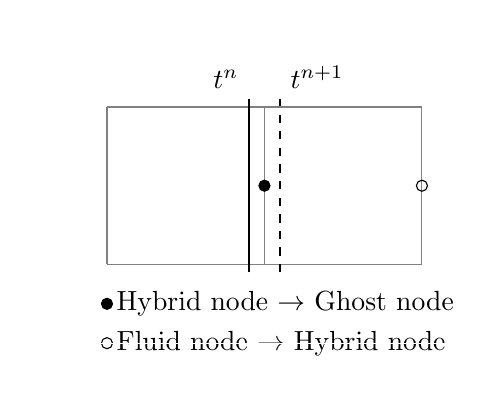
\begin{tikzpicture}
%grid
%horizontal
\draw[gray, thin] (-2,1) -- (2,1);
\draw[gray, thin] (-2,-1) -- (2,-1);
%vertical
\draw[gray, thin] (-2,1) -- (-2,-1);
\draw[gray, thin] (0,1) -- (0,-1);
\draw[gray, thin] (2,1) -- (2,-1);
%body
\draw[black, thick] (-0.2,-1.1) -- (-0.2,1.1) node[anchor=south east] {$t^n$};
\draw[black, thick, dashed] (0.2,-1.1) -- (0.2,1.1) node[anchor=south west] {$t^{n+1}$};
%nodes
\draw [black] (2.0,0) circle (2pt); %fluid
\filldraw [black] (0,0) circle (2pt);%hybrid
%legend
\filldraw (-2,-1.5) circle (2pt) node[anchor=west] {Hybrid node $\rightarrow$ Ghost node};
\draw (-2,-2.0) circle (2pt) node[anchor=west] {Fluid node $\rightarrow$ Hybrid node};
%\node [anchor=north, align=center] at (-1,-1) {Hybrid node \\Ghost node};
%\node [anchor=north, align=center] at (1,-1) {Fluid node \\Hybrid node};
%\node [anchor=east] at (-2,-1.25) {$t^n$};
%\node [anchor=east] at (-2,-1.7) {$t^{n+1}$};

%anchors used to make the pictures align with each other
\draw[white] (2.5,-2) -- (-3.0,-2) -- (-3.0,2) -- (2.5,2) -- cycle;
\end{tikzpicture}
\end{document}
